\documentclass[twocolumn,aps,showpacs,superscriptaddress,prl]{revtex4}

\usepackage{amsmath,amssymb,graphicx}
\usepackage{bm}
\usepackage{algorithmic}
\usepackage{enumerate}
\usepackage{color}
\usepackage{stmaryrd}
\usepackage{times}
\def\comment#1{{\bf\color{red}#1}}
\def\cm#1{{\bf\color{red}#1}}


\newcommand{\W}{W} 
\newcommand{\pbc}{\pi}
\newcommand{\abc}{\overline{\pi}}
\newcommand{\lav}{\bm{\langle}}
\newcommand{\rav}{\bm{\rangle}}

\newcommand{\cJ}{{\cal J}}
\newcommand{\D}{\Gamma_{\ell}}
\newcommand{\PJ}{P_{\cal J}(q)}
\newcommand{\PD}{P(q)}

\newcommand{\T}{S}
\newcommand{\ratio}{\Gamma_s}


\begin{document}

\title{Calculation of Boundary Condition in the Migdal-Kadanoff Spin Glass and Size Chaos}


\author{Jeff Gertler}
\email{jgertler@physics.umass.edu}
\affiliation{Department of Physics, University of Massachusetts,
Amherst, Massachusetts 01003 USA}


\author{Jonathan Machta}
\email{machta@physics.umass.edu}
\affiliation{Department of Physics, University of Massachusetts,
Amherst, Massachusetts 01003 USA}
\affiliation{Santa Fe Institute, 1399 Hyde Park Road, Santa Fe, New Mexico
87501, USA}

\begin{abstract}

Abstract here

\end{abstract}

\pacs{75.50.Lk, 75.40.Mg, 05.50.+q, 64.60.-i}
\maketitle



\paragraph*{Boundary Condition Calculation} ---


% Parallel bonds
\begin{equation}
K' = K_1 + K_2
\label{eq:par}
\end{equation}

% Series bonds
\begin{equation}
K' = \frac{1}{2}\ln \Big(\frac{\cosh(K_1+K_2)}{\cosh(K_1-K_2)} \Big)
\label{eq:ser}
\end{equation}

% MKRG
\begin{equation}
K' = \frac{1}{2}\ln \Big(\frac{\cosh(K_1+K_2+K_3+K_4+K_5+K_6+K_7+K_8)}{\cosh(K_1+K_2+K_3+K_4-K_5-K_6-K_7-K_8)} \Big)
\label{eq:mkrg}
\end{equation}





%\begin{figure}[htb]
%\begin{center}
%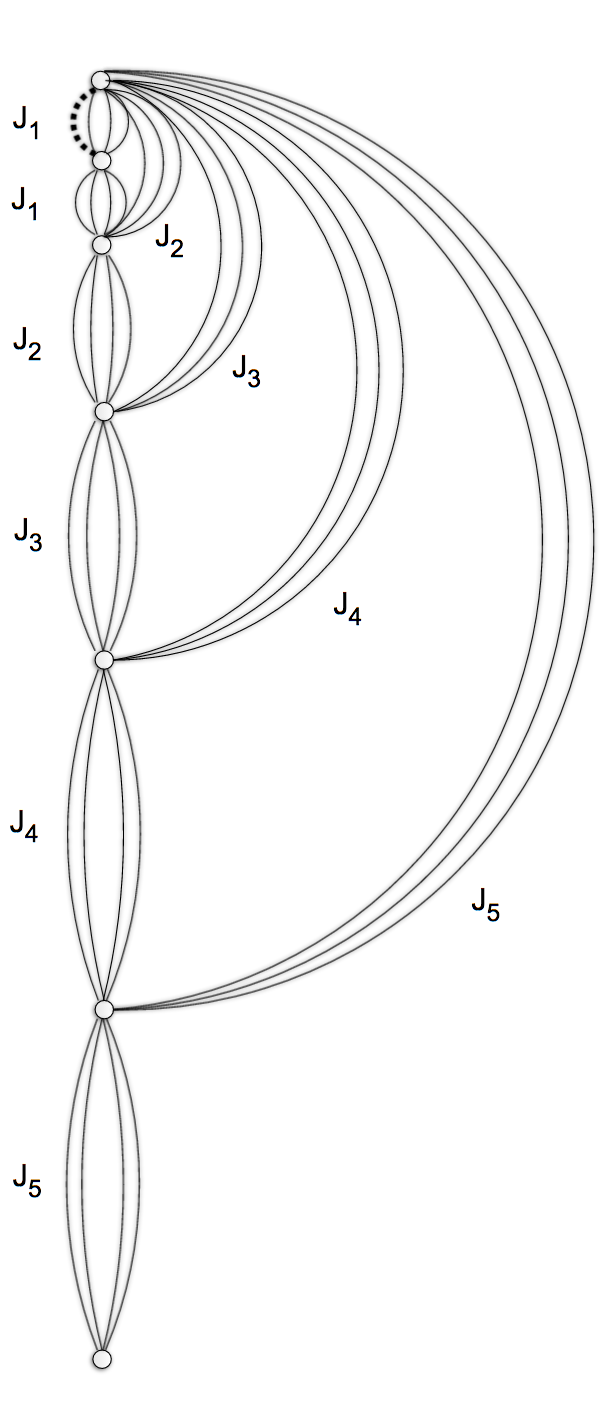
\includegraphics[width=0.5\columnwidth]{full_diag.png}
%\caption{
%Full Migdal-Kadanoff latice.
%}
%\label{Pq3}
%\end{center}
%\end{figure}

%\begin{figure}[htb]
%\begin{center}
%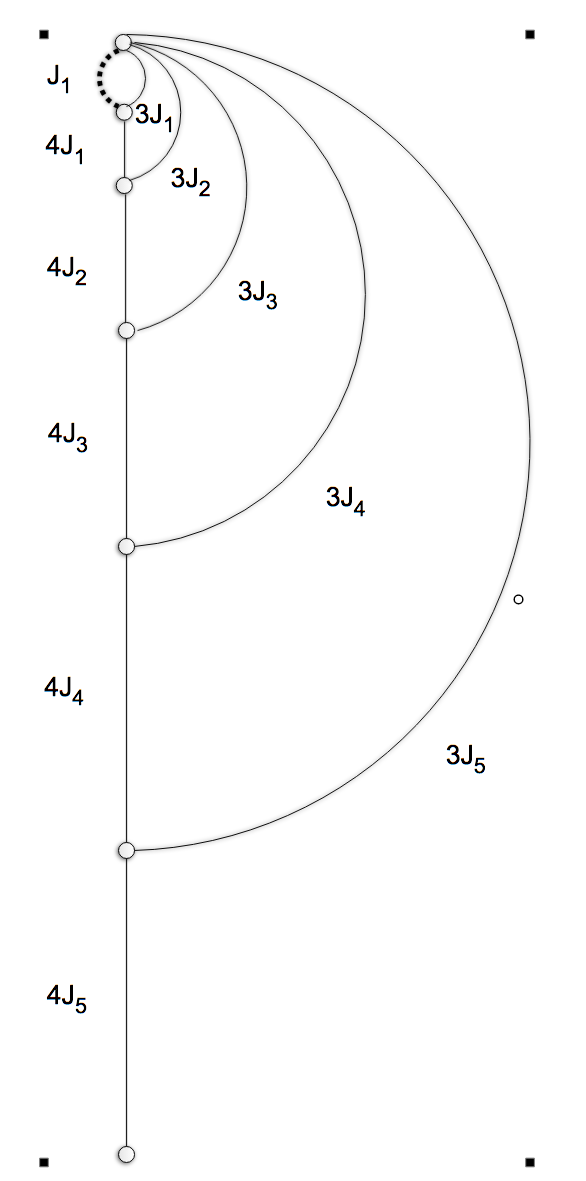
\includegraphics[width=0.5\columnwidth]{reduced_diag.png}
%\caption{
%Reduced Migdal-Kadanoff through parallel equation.
%}
%\label{Pq3}
%\end{center}
%\end{figure}

% BC Calculation
\begin{equation}
\begin{split}
K_{BC} = 3K_1 + (4K_1:(3K_2 + 4K_2:(3K_3 \\
+ 4K_3:(3K_4 + 4K_4:(3K_5+ ...)))))
\end{split}
\label{eq:bc}
\end{equation}


\paragraph*{Size Chaos} ---

% Correlation function
\begin{equation}
F(n) = | \tanh(K_n) - \tanh(K_{\inf}) |
\label{eq:cor}
\end{equation}


\paragraph*{Necklace Analytics} ---\\
Let $B_0$ be the boundary condition for a finite subsystem through a supersystem one level larger. Let $h$ be the largest level of the supersystem. To calculate the BC through a larger supersystem by one level we can do a replacement on the elements of $B_0$ as followed:
\begin{equation}
B_0 = (n-1)\cdot K_{h} \rightarrow B_0 = (n-1)\cdot K_h + n \cdot K_h:(n-1)\cdot K_{h+1}
\end{equation}
Let $G$, $G'$, and $G''$ be values drawn from the 0t distribution of the necklace MKRG distribution scaled to variance 1. The general replacement equation above can be rewritten as:
\begin{equation}
\sqrt{n} G \rightarrow \sqrt{n} G + \sqrt{n} G': \sqrt{n} \tau G'')
\end{equation}
Note that $n-1=n$ when $n>>1$ and $\tau$ is the scaling value for the necklace MKRG. This can be simplified to:
\begin{equation}
G \rightarrow G + sgn(G G)G
\end{equation}

\paragraph*{Diamond Analytics} ---\\
Let $B_0$ and $h$ be the same as above. 
\begin{equation}
B_0 = K_0 :(n-1)\cdot (K_0:K_0)
\end{equation}
The replacement rule is:
\begin{equation}
B_0 = (n-1)\cdot(K_h:K_h) \rightarrow
B_0 = (n-1)\cdot(K_h:K_h) + K_{h+1} : ((n-1)\cdot(K_{h+1}:K_{h+1}))
\end{equation}
Again $G$, $G'$, $G''$, $G'''$, $G''''$ are drawn from the diamond MKRG distribution scaled to variance 1.
\begin{equation}
\sqrt{n}(G:G') \rightarrow \sqrt{n}(G:G')+ \tau \sqrt{n}(G'':(\sqrt{n} G''':G''''))
\end{equation}
This reduces to:
\begin{equation}
G:G' \rightarrow G:G' + \tau [G'': (\sqrt{n}G''':G'''')]
\end{equation}
\begin{equation}
H \equiv G:G'
\end{equation}
\begin{equation}
H \rightarrow H+ \tau[G:\sqrt{n} H']
\end{equation}
\begin{equation}
X \equiv \frac{G:G'}{\sqrt{VAR(G:G')}} = \frac{H}{\tau}
\end{equation}
\begin{equation}
X \tau \rightarrow X\tau + \tau(G:\sqrt{n} \tau X')
\end{equation}
\begin{equation}
X \rightarrow X + (G:\sqrt{n}\tau X')
\end{equation}
\begin{equation}
X \rightarrow X + sgn(GX')G
\end{equation}

\begin{acknowledgments}



\end{acknowledgments}

\bibliographystyle{apsrevtitle}
\bibliography{refs}

\end{document}
